% Options for packages loaded elsewhere
\PassOptionsToPackage{unicode}{hyperref}
\PassOptionsToPackage{hyphens}{url}
%
\documentclass[
  ignorenonframetext,
]{beamer}
\usepackage{pgfpages}
\setbeamertemplate{caption}[numbered]
\setbeamertemplate{caption label separator}{: }
\setbeamercolor{caption name}{fg=normal text.fg}
\beamertemplatenavigationsymbolsempty
% Prevent slide breaks in the middle of a paragraph
\widowpenalties 1 10000
\raggedbottom
\setbeamertemplate{part page}{
  \centering
  \begin{beamercolorbox}[sep=16pt,center]{part title}
    \usebeamerfont{part title}\insertpart\par
  \end{beamercolorbox}
}
\setbeamertemplate{section page}{
  \centering
  \begin{beamercolorbox}[sep=12pt,center]{part title}
    \usebeamerfont{section title}\insertsection\par
  \end{beamercolorbox}
}
\setbeamertemplate{subsection page}{
  \centering
  \begin{beamercolorbox}[sep=8pt,center]{part title}
    \usebeamerfont{subsection title}\insertsubsection\par
  \end{beamercolorbox}
}
\AtBeginPart{
  \frame{\partpage}
}
\AtBeginSection{
  \ifbibliography
  \else
    \frame{\sectionpage}
  \fi
}
\AtBeginSubsection{
  \frame{\subsectionpage}
}
\usepackage{lmodern}
\usepackage{amssymb,amsmath}
\usepackage{ifxetex,ifluatex}
\ifnum 0\ifxetex 1\fi\ifluatex 1\fi=0 % if pdftex
  \usepackage[T1]{fontenc}
  \usepackage[utf8]{inputenc}
  \usepackage{textcomp} % provide euro and other symbols
\else % if luatex or xetex
  \usepackage{unicode-math}
  \defaultfontfeatures{Scale=MatchLowercase}
  \defaultfontfeatures[\rmfamily]{Ligatures=TeX,Scale=1}
\fi
% Use upquote if available, for straight quotes in verbatim environments
\IfFileExists{upquote.sty}{\usepackage{upquote}}{}
\IfFileExists{microtype.sty}{% use microtype if available
  \usepackage[]{microtype}
  \UseMicrotypeSet[protrusion]{basicmath} % disable protrusion for tt fonts
}{}
\makeatletter
\@ifundefined{KOMAClassName}{% if non-KOMA class
  \IfFileExists{parskip.sty}{%
    \usepackage{parskip}
  }{% else
    \setlength{\parindent}{0pt}
    \setlength{\parskip}{6pt plus 2pt minus 1pt}}
}{% if KOMA class
  \KOMAoptions{parskip=half}}
\makeatother
\usepackage{xcolor}
\IfFileExists{xurl.sty}{\usepackage{xurl}}{} % add URL line breaks if available
\IfFileExists{bookmark.sty}{\usepackage{bookmark}}{\usepackage{hyperref}}
\hypersetup{
  pdftitle={Module 9: Logistic Regression},
  pdfauthor={Rebecca C. Steorts},
  hidelinks,
  pdfcreator={LaTeX via pandoc}}
\urlstyle{same} % disable monospaced font for URLs
\newif\ifbibliography
\usepackage{color}
\usepackage{fancyvrb}
\newcommand{\VerbBar}{|}
\newcommand{\VERB}{\Verb[commandchars=\\\{\}]}
\DefineVerbatimEnvironment{Highlighting}{Verbatim}{commandchars=\\\{\}}
% Add ',fontsize=\small' for more characters per line
\usepackage{framed}
\definecolor{shadecolor}{RGB}{248,248,248}
\newenvironment{Shaded}{\begin{snugshade}}{\end{snugshade}}
\newcommand{\AlertTok}[1]{\textcolor[rgb]{0.94,0.16,0.16}{#1}}
\newcommand{\AnnotationTok}[1]{\textcolor[rgb]{0.56,0.35,0.01}{\textbf{\textit{#1}}}}
\newcommand{\AttributeTok}[1]{\textcolor[rgb]{0.77,0.63,0.00}{#1}}
\newcommand{\BaseNTok}[1]{\textcolor[rgb]{0.00,0.00,0.81}{#1}}
\newcommand{\BuiltInTok}[1]{#1}
\newcommand{\CharTok}[1]{\textcolor[rgb]{0.31,0.60,0.02}{#1}}
\newcommand{\CommentTok}[1]{\textcolor[rgb]{0.56,0.35,0.01}{\textit{#1}}}
\newcommand{\CommentVarTok}[1]{\textcolor[rgb]{0.56,0.35,0.01}{\textbf{\textit{#1}}}}
\newcommand{\ConstantTok}[1]{\textcolor[rgb]{0.00,0.00,0.00}{#1}}
\newcommand{\ControlFlowTok}[1]{\textcolor[rgb]{0.13,0.29,0.53}{\textbf{#1}}}
\newcommand{\DataTypeTok}[1]{\textcolor[rgb]{0.13,0.29,0.53}{#1}}
\newcommand{\DecValTok}[1]{\textcolor[rgb]{0.00,0.00,0.81}{#1}}
\newcommand{\DocumentationTok}[1]{\textcolor[rgb]{0.56,0.35,0.01}{\textbf{\textit{#1}}}}
\newcommand{\ErrorTok}[1]{\textcolor[rgb]{0.64,0.00,0.00}{\textbf{#1}}}
\newcommand{\ExtensionTok}[1]{#1}
\newcommand{\FloatTok}[1]{\textcolor[rgb]{0.00,0.00,0.81}{#1}}
\newcommand{\FunctionTok}[1]{\textcolor[rgb]{0.00,0.00,0.00}{#1}}
\newcommand{\ImportTok}[1]{#1}
\newcommand{\InformationTok}[1]{\textcolor[rgb]{0.56,0.35,0.01}{\textbf{\textit{#1}}}}
\newcommand{\KeywordTok}[1]{\textcolor[rgb]{0.13,0.29,0.53}{\textbf{#1}}}
\newcommand{\NormalTok}[1]{#1}
\newcommand{\OperatorTok}[1]{\textcolor[rgb]{0.81,0.36,0.00}{\textbf{#1}}}
\newcommand{\OtherTok}[1]{\textcolor[rgb]{0.56,0.35,0.01}{#1}}
\newcommand{\PreprocessorTok}[1]{\textcolor[rgb]{0.56,0.35,0.01}{\textit{#1}}}
\newcommand{\RegionMarkerTok}[1]{#1}
\newcommand{\SpecialCharTok}[1]{\textcolor[rgb]{0.00,0.00,0.00}{#1}}
\newcommand{\SpecialStringTok}[1]{\textcolor[rgb]{0.31,0.60,0.02}{#1}}
\newcommand{\StringTok}[1]{\textcolor[rgb]{0.31,0.60,0.02}{#1}}
\newcommand{\VariableTok}[1]{\textcolor[rgb]{0.00,0.00,0.00}{#1}}
\newcommand{\VerbatimStringTok}[1]{\textcolor[rgb]{0.31,0.60,0.02}{#1}}
\newcommand{\WarningTok}[1]{\textcolor[rgb]{0.56,0.35,0.01}{\textbf{\textit{#1}}}}
\usepackage{graphicx,grffile}
\makeatletter
\def\maxwidth{\ifdim\Gin@nat@width>\linewidth\linewidth\else\Gin@nat@width\fi}
\def\maxheight{\ifdim\Gin@nat@height>\textheight\textheight\else\Gin@nat@height\fi}
\makeatother
% Scale images if necessary, so that they will not overflow the page
% margins by default, and it is still possible to overwrite the defaults
% using explicit options in \includegraphics[width, height, ...]{}
\setkeys{Gin}{width=\maxwidth,height=\maxheight,keepaspectratio}
% Set default figure placement to htbp
\makeatletter
\def\fps@figure{htbp}
\makeatother
\setlength{\emergencystretch}{3em} % prevent overfull lines
\providecommand{\tightlist}{%
  \setlength{\itemsep}{0pt}\setlength{\parskip}{0pt}}
\setcounter{secnumdepth}{-\maxdimen} % remove section numbering
% Custom definitions
% To use this customization file, insert the line "% Custom definitions
% To use this customization file, insert the line "% Custom definitions
% To use this customization file, insert the line "% Custom definitions
% To use this customization file, insert the line "\input{custom}" in the header of the tex file.

% Formatting

\tolerance=1000
\usepackage[margin=1in]{geometry}


% Packages

% \usepackage{amssymb,latexsym}
\usepackage{amssymb,amsfonts,amsmath,latexsym,amsthm}
\usepackage[usenames,dvipsnames]{color}
\usepackage[]{graphicx}
\usepackage[space]{grffile}
\usepackage{mathrsfs}   % fancy math font
% \usepackage[font=small,skip=0pt]{caption}
\usepackage[skip=0pt]{caption}
\usepackage{subcaption}
\usepackage{verbatim}
\usepackage{url}
\usepackage{bm}
\usepackage{dsfont}
\usepackage{extarrows}
\usepackage{multirow}
% \usepackage{wrapfig}
% \usepackage{epstopdf}
\usepackage{rotating}
\usepackage{tikz}
\usetikzlibrary{fit}					% fitting shapes to coordinates
%\usetikzlibrary{backgrounds}	% drawing the background after the foreground


% \usepackage[dvipdfm,colorlinks,citecolor=blue,linkcolor=blue,urlcolor=blue]{hyperref}
\usepackage[colorlinks,citecolor=blue,linkcolor=blue,urlcolor=blue]{hyperref}
%\usepackage{hyperref}
\usepackage[authoryear,round]{natbib}


%  Theorems, etc.

\theoremstyle{plain}
\newtheorem{theorem}{Theorem}[section]
\newtheorem{corollary}[theorem]{Corollary}
\newtheorem{lemma}[theorem]{Lemma}
\newtheorem{proposition}[theorem]{Proposition}
\newtheorem{condition}[theorem]{Condition}
% \newtheorem{conditions}[theorem]{Conditions}

\theoremstyle{definition}
\newtheorem{definition}[theorem]{Definition}
% \newtheorem*{unnumbered-definition}{Definition}
\newtheorem{example}[theorem]{Example}
\theoremstyle{remark}
\newtheorem*{remark}{Remark}
\numberwithin{equation}{section}




% Document-specific shortcuts
\newcommand{\btheta}{{\bm\theta}}
\newcommand{\bbtheta}{{\pmb{\bm\theta}}}

\newcommand{\commentary}[1]{\ifx\showcommentary\undefined\else \emph{#1}\fi}

\newcommand{\term}[1]{\textit{\textbf{#1}}}

% Math shortcuts

% Probability distributions
\DeclareMathOperator*{\Exp}{Exp}
\DeclareMathOperator*{\TExp}{TExp}
\DeclareMathOperator*{\Bernoulli}{Bernoulli}
\DeclareMathOperator*{\Beta}{Beta}
\DeclareMathOperator*{\Ga}{Gamma}
\DeclareMathOperator*{\TGamma}{TGamma}
\DeclareMathOperator*{\Poisson}{Poisson}
\DeclareMathOperator*{\Binomial}{Binomial}
\DeclareMathOperator*{\NormalGamma}{NormalGamma}
\DeclareMathOperator*{\InvGamma}{InvGamma}
\DeclareMathOperator*{\Cauchy}{Cauchy}
\DeclareMathOperator*{\Uniform}{Uniform}
\DeclareMathOperator*{\Gumbel}{Gumbel}
\DeclareMathOperator*{\Pareto}{Pareto}
\DeclareMathOperator*{\Mono}{Mono}
\DeclareMathOperator*{\Geometric}{Geometric}
\DeclareMathOperator*{\Wishart}{Wishart}

% Math operators
\DeclareMathOperator*{\argmin}{arg\,min}
\DeclareMathOperator*{\argmax}{arg\,max}
\DeclareMathOperator*{\Cov}{Cov}
\DeclareMathOperator*{\diag}{diag}
\DeclareMathOperator*{\median}{median}
\DeclareMathOperator*{\Vol}{Vol}

% Math characters
\newcommand{\R}{\mathbb{R}}
\newcommand{\Z}{\mathbb{Z}}
\newcommand{\E}{\mathbb{E}}
\renewcommand{\Pr}{\mathbb{P}}
\newcommand{\I}{\mathds{1}}
\newcommand{\V}{\mathbb{V}}

\newcommand{\A}{\mathcal{A}}
\newcommand{\C}{\mathcal{C}}
\newcommand{\D}{\mathcal{D}}
\newcommand{\Hcal}{\mathcal{H}}
\newcommand{\M}{\mathcal{M}}
\newcommand{\N}{\mathcal{N}}
\newcommand{\X}{\mathcal{X}}
\newcommand{\Zcal}{\mathcal{Z}}
\renewcommand{\P}{\mathcal{P}}

\newcommand{\T}{\mathtt{T}}
\renewcommand{\emptyset}{\varnothing}


% Miscellaneous commands
\newcommand{\iid}{\stackrel{\mathrm{iid}}{\sim}}
\newcommand{\matrixsmall}[1]{\bigl(\begin{smallmatrix}#1\end{smallmatrix} \bigr)}

\newcommand{\items}[1]{\begin{itemize} #1 \end{itemize}}

\newcommand{\todo}[1]{\emph{\textcolor{red}{(#1)}}}

\newcommand{\branch}[4]{
\left\{
	\begin{array}{ll}
		#1  & \mbox{if } #2 \\
		#3 & \mbox{if } #4
	\end{array}
\right.
}

% approximately proportional to
\def\app#1#2{%
  \mathrel{%
    \setbox0=\hbox{$#1\sim$}%
    \setbox2=\hbox{%
      \rlap{\hbox{$#1\propto$}}%
      \lower1.3\ht0\box0%
    }%
    \raise0.25\ht2\box2%
  }%
}
\def\approxprop{\mathpalette\app\relax}

% \newcommand{\approptoinn}[2]{\mathrel{\vcenter{
  % \offinterlineskip\halign{\hfil$##$\cr
    % #1\propto\cr\noalign{\kern2pt}#1\sim\cr\noalign{\kern-2pt}}}}}

% \newcommand{\approxpropto}{\mathpalette\approptoinn\relax}





" in the header of the tex file.

% Formatting

\tolerance=1000
\usepackage[margin=1in]{geometry}


% Packages

% \usepackage{amssymb,latexsym}
\usepackage{amssymb,amsfonts,amsmath,latexsym,amsthm}
\usepackage[usenames,dvipsnames]{color}
\usepackage[]{graphicx}
\usepackage[space]{grffile}
\usepackage{mathrsfs}   % fancy math font
% \usepackage[font=small,skip=0pt]{caption}
\usepackage[skip=0pt]{caption}
\usepackage{subcaption}
\usepackage{verbatim}
\usepackage{url}
\usepackage{bm}
\usepackage{dsfont}
\usepackage{extarrows}
\usepackage{multirow}
% \usepackage{wrapfig}
% \usepackage{epstopdf}
\usepackage{rotating}
\usepackage{tikz}
\usetikzlibrary{fit}					% fitting shapes to coordinates
%\usetikzlibrary{backgrounds}	% drawing the background after the foreground


% \usepackage[dvipdfm,colorlinks,citecolor=blue,linkcolor=blue,urlcolor=blue]{hyperref}
\usepackage[colorlinks,citecolor=blue,linkcolor=blue,urlcolor=blue]{hyperref}
%\usepackage{hyperref}
\usepackage[authoryear,round]{natbib}


%  Theorems, etc.

\theoremstyle{plain}
\newtheorem{theorem}{Theorem}[section]
\newtheorem{corollary}[theorem]{Corollary}
\newtheorem{lemma}[theorem]{Lemma}
\newtheorem{proposition}[theorem]{Proposition}
\newtheorem{condition}[theorem]{Condition}
% \newtheorem{conditions}[theorem]{Conditions}

\theoremstyle{definition}
\newtheorem{definition}[theorem]{Definition}
% \newtheorem*{unnumbered-definition}{Definition}
\newtheorem{example}[theorem]{Example}
\theoremstyle{remark}
\newtheorem*{remark}{Remark}
\numberwithin{equation}{section}




% Document-specific shortcuts
\newcommand{\btheta}{{\bm\theta}}
\newcommand{\bbtheta}{{\pmb{\bm\theta}}}

\newcommand{\commentary}[1]{\ifx\showcommentary\undefined\else \emph{#1}\fi}

\newcommand{\term}[1]{\textit{\textbf{#1}}}

% Math shortcuts

% Probability distributions
\DeclareMathOperator*{\Exp}{Exp}
\DeclareMathOperator*{\TExp}{TExp}
\DeclareMathOperator*{\Bernoulli}{Bernoulli}
\DeclareMathOperator*{\Beta}{Beta}
\DeclareMathOperator*{\Ga}{Gamma}
\DeclareMathOperator*{\TGamma}{TGamma}
\DeclareMathOperator*{\Poisson}{Poisson}
\DeclareMathOperator*{\Binomial}{Binomial}
\DeclareMathOperator*{\NormalGamma}{NormalGamma}
\DeclareMathOperator*{\InvGamma}{InvGamma}
\DeclareMathOperator*{\Cauchy}{Cauchy}
\DeclareMathOperator*{\Uniform}{Uniform}
\DeclareMathOperator*{\Gumbel}{Gumbel}
\DeclareMathOperator*{\Pareto}{Pareto}
\DeclareMathOperator*{\Mono}{Mono}
\DeclareMathOperator*{\Geometric}{Geometric}
\DeclareMathOperator*{\Wishart}{Wishart}

% Math operators
\DeclareMathOperator*{\argmin}{arg\,min}
\DeclareMathOperator*{\argmax}{arg\,max}
\DeclareMathOperator*{\Cov}{Cov}
\DeclareMathOperator*{\diag}{diag}
\DeclareMathOperator*{\median}{median}
\DeclareMathOperator*{\Vol}{Vol}

% Math characters
\newcommand{\R}{\mathbb{R}}
\newcommand{\Z}{\mathbb{Z}}
\newcommand{\E}{\mathbb{E}}
\renewcommand{\Pr}{\mathbb{P}}
\newcommand{\I}{\mathds{1}}
\newcommand{\V}{\mathbb{V}}

\newcommand{\A}{\mathcal{A}}
\newcommand{\C}{\mathcal{C}}
\newcommand{\D}{\mathcal{D}}
\newcommand{\Hcal}{\mathcal{H}}
\newcommand{\M}{\mathcal{M}}
\newcommand{\N}{\mathcal{N}}
\newcommand{\X}{\mathcal{X}}
\newcommand{\Zcal}{\mathcal{Z}}
\renewcommand{\P}{\mathcal{P}}

\newcommand{\T}{\mathtt{T}}
\renewcommand{\emptyset}{\varnothing}


% Miscellaneous commands
\newcommand{\iid}{\stackrel{\mathrm{iid}}{\sim}}
\newcommand{\matrixsmall}[1]{\bigl(\begin{smallmatrix}#1\end{smallmatrix} \bigr)}

\newcommand{\items}[1]{\begin{itemize} #1 \end{itemize}}

\newcommand{\todo}[1]{\emph{\textcolor{red}{(#1)}}}

\newcommand{\branch}[4]{
\left\{
	\begin{array}{ll}
		#1  & \mbox{if } #2 \\
		#3 & \mbox{if } #4
	\end{array}
\right.
}

% approximately proportional to
\def\app#1#2{%
  \mathrel{%
    \setbox0=\hbox{$#1\sim$}%
    \setbox2=\hbox{%
      \rlap{\hbox{$#1\propto$}}%
      \lower1.3\ht0\box0%
    }%
    \raise0.25\ht2\box2%
  }%
}
\def\approxprop{\mathpalette\app\relax}

% \newcommand{\approptoinn}[2]{\mathrel{\vcenter{
  % \offinterlineskip\halign{\hfil$##$\cr
    % #1\propto\cr\noalign{\kern2pt}#1\sim\cr\noalign{\kern-2pt}}}}}

% \newcommand{\approxpropto}{\mathpalette\approptoinn\relax}





" in the header of the tex file.

% Formatting

\tolerance=1000
\usepackage[margin=1in]{geometry}


% Packages

% \usepackage{amssymb,latexsym}
\usepackage{amssymb,amsfonts,amsmath,latexsym,amsthm}
\usepackage[usenames,dvipsnames]{color}
\usepackage[]{graphicx}
\usepackage[space]{grffile}
\usepackage{mathrsfs}   % fancy math font
% \usepackage[font=small,skip=0pt]{caption}
\usepackage[skip=0pt]{caption}
\usepackage{subcaption}
\usepackage{verbatim}
\usepackage{url}
\usepackage{bm}
\usepackage{dsfont}
\usepackage{extarrows}
\usepackage{multirow}
% \usepackage{wrapfig}
% \usepackage{epstopdf}
\usepackage{rotating}
\usepackage{tikz}
\usetikzlibrary{fit}					% fitting shapes to coordinates
%\usetikzlibrary{backgrounds}	% drawing the background after the foreground


% \usepackage[dvipdfm,colorlinks,citecolor=blue,linkcolor=blue,urlcolor=blue]{hyperref}
\usepackage[colorlinks,citecolor=blue,linkcolor=blue,urlcolor=blue]{hyperref}
%\usepackage{hyperref}
\usepackage[authoryear,round]{natbib}


%  Theorems, etc.

\theoremstyle{plain}
\newtheorem{theorem}{Theorem}[section]
\newtheorem{corollary}[theorem]{Corollary}
\newtheorem{lemma}[theorem]{Lemma}
\newtheorem{proposition}[theorem]{Proposition}
\newtheorem{condition}[theorem]{Condition}
% \newtheorem{conditions}[theorem]{Conditions}

\theoremstyle{definition}
\newtheorem{definition}[theorem]{Definition}
% \newtheorem*{unnumbered-definition}{Definition}
\newtheorem{example}[theorem]{Example}
\theoremstyle{remark}
\newtheorem*{remark}{Remark}
\numberwithin{equation}{section}




% Document-specific shortcuts
\newcommand{\btheta}{{\bm\theta}}
\newcommand{\bbtheta}{{\pmb{\bm\theta}}}

\newcommand{\commentary}[1]{\ifx\showcommentary\undefined\else \emph{#1}\fi}

\newcommand{\term}[1]{\textit{\textbf{#1}}}

% Math shortcuts

% Probability distributions
\DeclareMathOperator*{\Exp}{Exp}
\DeclareMathOperator*{\TExp}{TExp}
\DeclareMathOperator*{\Bernoulli}{Bernoulli}
\DeclareMathOperator*{\Beta}{Beta}
\DeclareMathOperator*{\Ga}{Gamma}
\DeclareMathOperator*{\TGamma}{TGamma}
\DeclareMathOperator*{\Poisson}{Poisson}
\DeclareMathOperator*{\Binomial}{Binomial}
\DeclareMathOperator*{\NormalGamma}{NormalGamma}
\DeclareMathOperator*{\InvGamma}{InvGamma}
\DeclareMathOperator*{\Cauchy}{Cauchy}
\DeclareMathOperator*{\Uniform}{Uniform}
\DeclareMathOperator*{\Gumbel}{Gumbel}
\DeclareMathOperator*{\Pareto}{Pareto}
\DeclareMathOperator*{\Mono}{Mono}
\DeclareMathOperator*{\Geometric}{Geometric}
\DeclareMathOperator*{\Wishart}{Wishart}

% Math operators
\DeclareMathOperator*{\argmin}{arg\,min}
\DeclareMathOperator*{\argmax}{arg\,max}
\DeclareMathOperator*{\Cov}{Cov}
\DeclareMathOperator*{\diag}{diag}
\DeclareMathOperator*{\median}{median}
\DeclareMathOperator*{\Vol}{Vol}

% Math characters
\newcommand{\R}{\mathbb{R}}
\newcommand{\Z}{\mathbb{Z}}
\newcommand{\E}{\mathbb{E}}
\renewcommand{\Pr}{\mathbb{P}}
\newcommand{\I}{\mathds{1}}
\newcommand{\V}{\mathbb{V}}

\newcommand{\A}{\mathcal{A}}
\newcommand{\C}{\mathcal{C}}
\newcommand{\D}{\mathcal{D}}
\newcommand{\Hcal}{\mathcal{H}}
\newcommand{\M}{\mathcal{M}}
\newcommand{\N}{\mathcal{N}}
\newcommand{\X}{\mathcal{X}}
\newcommand{\Zcal}{\mathcal{Z}}
\renewcommand{\P}{\mathcal{P}}

\newcommand{\T}{\mathtt{T}}
\renewcommand{\emptyset}{\varnothing}


% Miscellaneous commands
\newcommand{\iid}{\stackrel{\mathrm{iid}}{\sim}}
\newcommand{\matrixsmall}[1]{\bigl(\begin{smallmatrix}#1\end{smallmatrix} \bigr)}

\newcommand{\items}[1]{\begin{itemize} #1 \end{itemize}}

\newcommand{\todo}[1]{\emph{\textcolor{red}{(#1)}}}

\newcommand{\branch}[4]{
\left\{
	\begin{array}{ll}
		#1  & \mbox{if } #2 \\
		#3 & \mbox{if } #4
	\end{array}
\right.
}

% approximately proportional to
\def\app#1#2{%
  \mathrel{%
    \setbox0=\hbox{$#1\sim$}%
    \setbox2=\hbox{%
      \rlap{\hbox{$#1\propto$}}%
      \lower1.3\ht0\box0%
    }%
    \raise0.25\ht2\box2%
  }%
}
\def\approxprop{\mathpalette\app\relax}

% \newcommand{\approptoinn}[2]{\mathrel{\vcenter{
  % \offinterlineskip\halign{\hfil$##$\cr
    % #1\propto\cr\noalign{\kern2pt}#1\sim\cr\noalign{\kern-2pt}}}}}

% \newcommand{\approxpropto}{\mathpalette\approptoinn\relax}





" in the header of the tex file.

% Formatting

\setbeamertemplate{navigation symbols}{}
\setbeamertemplate{footline}[page number]

\usepackage{bbm}
% Packages
\usepackage{amssymb,amsfonts,amsmath,latexsym,amsthm}
%\usepackage[usenames,dvipsnames]{color}
%\usepackage[]{graphicx}
%\usepackage[space]{grffile}
\usepackage{mathrsfs} 
 \usepackage{amssymb,latexsym}
\usepackage{amssymb,amsfonts,amsmath,latexsym,amsthm, bm}
%\usepackage[usenames,dvipsnames]{color}
%\usepackage[]{graphicx}
%\usepackage[space]{grffile}
\usepackage{mathrsfs}   % fancy math font
% \usepackage[font=small,skip=0pt]{caption}
%\usepackage[skip=0pt]{caption}
%\usepackage{subcaption}
%\usepackage{verbatim}
%\usepackage{url}
%\usepackage{bm}
\usepackage{dsfont}
\usepackage{multirow}
%\usepackage{extarrows}
%\usepackage{multirow}
%% \usepackage{wrapfig}
%% \usepackage{epstopdf}
%\usepackage{rotating}
%\usepackage{tikz}
%\usetikzlibrary{fit}					% fitting shapes to coordinates
%\usetikzlibrary{backgrounds}	% drawing the background after the foreground


% \usepackage[dvipdfm,colorlinks,citecolor=blue,linkcolor=blue,urlcolor=blue]{hyperref}
%\usepackage[colorlinks,citecolor=blue,linkcolor=blue,urlcolor=blue]{hyperref}
%%\usepackage{hyperref}
%\usepackage[authoryear,round]{natbib}


%  Theorems, etc.

%\theoremstyle{plain}
%\newtheorem{theorem}{Theorem}[section]
%\newtheorem{corollary}[theorem]{Corollary}
%\newtheorem{lemma}[theorem]{Lemma}
%\newtheorem{proposition}[theorem]{Proposition}
%\newtheorem{condition}[theorem]{Condition}
% \newtheorem{conditions}[theorem]{Conditions}

%\theoremstyle{definition}
%\newtheorem{definition}[theorem]{Definition}
%% \newtheorem*{unnumbered-definition}{Definition}
%\newtheorem{example}[theorem]{Example}
%\theoremstyle{remark}
%\newtheorem*{remark}{Remark}
%\numberwithin{equation}{section}

\newcommand{\bx}   {\bm{x}}
\newcommand{\bY}   {\bm{Y}}
\newcommand{\by}   {\bm{y}}

\newcommand{\hbeta}   {\hat{\beta}}
\newcommand{\hy}   {\hat{y}}


% Document-specific shortcuts
\newcommand{\btheta}{{\bm\theta}}
\newcommand{\bbtheta}{{\pmb{\bm\theta}}}

\newcommand{\commentary}[1]{\ifx\showcommentary\undefined\else \emph{#1}\fi}

\newcommand{\term}[1]{\textit{\textbf{#1}}}

% Math shortcuts

% Probability distributions
\DeclareMathOperator*{\Exp}{Exp}
\DeclareMathOperator*{\TExp}{TExp}
\DeclareMathOperator*{\Bernoulli}{Bernoulli}
\DeclareMathOperator*{\Beta}{Beta}
\DeclareMathOperator*{\Ga}{Gamma}
\DeclareMathOperator*{\TGamma}{TGamma}
\DeclareMathOperator*{\Poisson}{Poisson}
\DeclareMathOperator*{\Binomial}{Binomial}
\DeclareMathOperator*{\NormalGamma}{NormalGamma}
\DeclareMathOperator*{\InvGamma}{InvGamma}
\DeclareMathOperator*{\Cauchy}{Cauchy}
\DeclareMathOperator*{\Uniform}{Uniform}
\DeclareMathOperator*{\Gumbel}{Gumbel}
\DeclareMathOperator*{\Pareto}{Pareto}
\DeclareMathOperator*{\Mono}{Mono}
\DeclareMathOperator*{\Geometric}{Geometric}
\DeclareMathOperator*{\Wishart}{Wishart}

% Math operators
\DeclareMathOperator*{\argmin}{arg\,min}
\DeclareMathOperator*{\argmax}{arg\,max}
\DeclareMathOperator*{\Cov}{Cov}
\DeclareMathOperator*{\diag}{diag}
\DeclareMathOperator*{\median}{median}
\DeclareMathOperator*{\Vol}{Vol}

% Math characters
\newcommand{\R}{\mathbb{R}}
\newcommand{\Z}{\mathbb{Z}}
\newcommand{\E}{\mathbb{E}}
\renewcommand{\Pr}{\mathbb{P}}
\newcommand{\I}{\mathds{1}}
\newcommand{\V}{\mathbb{V}}
\newcommand{\bbeta}{\bm{\beta}}

\newcommand{\A}{\mathcal{A}}
%\newcommand{\C}{\mathcal{C}}
\newcommand{\D}{\mathcal{D}}
\newcommand{\Hcal}{\mathcal{H}}
\newcommand{\M}{\mathcal{M}}
\newcommand{\N}{\mathcal{N}}
\newcommand{\X}{\mathcal{X}}
\newcommand{\Zcal}{\mathcal{Z}}
\renewcommand{\P}{\mathcal{P}}


\newcommand{\T}{\mathtt{T}}
\renewcommand{\emptyset}{\varnothing}

\newcommand{\bmu}{\bm{\mu}}
\newcommand{\bX}   {\bm{X}}
\newcommand{\sig}   {\Sigma}
%\newcommand{\X}{\ensuremath{\mathbf{x}}}
%\newcommand{\w}{\ensuremath{\mathbf{w}}}
%\newcommand{\h}{\ensuremath{\mathbf{h}}}
%\newcommand{\V}{\ensuremath{\mathbf{v}}}
%\newcommand{\cov}{\text{Cov}}
\newcommand{\var}{\text{Var}}
\newcommand{\Var}{\text{Var}}



% Miscellaneous commands
\newcommand{\iid}{\stackrel{\mathrm{iid}}{\sim}}
\newcommand{\matrixsmall}[1]{\bigl(\begin{smallmatrix}#1\end{smallmatrix} \bigr)}

\newcommand{\items}[1]{\begin{itemize} #1 \end{itemize}}

\newcommand{\todo}[1]{\emph{\textcolor{red}{(#1)}}}

\newcommand{\branch}[4]{
\left\{
	\begin{array}{ll}
		#1  & \mbox{if } #2 \\
		#3 & \mbox{if } #4
	\end{array}
\right.
}

% approximately proportional to
\def\app#1#2{%
  \mathrel{%
    \setbox0=\hbox{$#1\sim$}%
    \setbox2=\hbox{%
      \rlap{\hbox{$#1\propto$}}%
      \lower1.3\ht0\box0%
    }%
    \raise0.25\ht2\box2%
  }%
}
\def\approxprop{\mathpalette\app\relax}

% \newcommand{\approptoinn}[2]{\mathrel{\vcenter{
  % \offinterlineskip\halign{\hfil$##$\cr
    % #1\propto\cr\noalign{\kern2pt}#1\sim\cr\noalign{\kern-2pt}}}}}

% \newcommand{\approxpropto}{\mathpalette\approptoinn\relax}

\title{Module 9: Logistic Regression}
\author{Rebecca C. Steorts}
\date{}

\begin{document}
\frame{\titlepage}

\begin{frame}{Agenda}
\protect\hypertarget{agenda}{}

\begin{itemize}
\tightlist
\item
  1986 Challenger explosion
\item
  Binary structure of the response data
\item
  Background: exponential families, generalized linear models (GLMs),
  logistic regression
\item
  Example on exponenital familes and GLMs
\item
  Bayesian logistic regression
\item
  Returning to the Challenger case study
\end{itemize}

\end{frame}

\begin{frame}{The Challenger Case Study}
\protect\hypertarget{the-challenger-case-study}{}

On 28 January 1986, the Space Shuttle Challenger broke apart, 73 seconds
into flight. All seven crew members died. The cause of the disaster was
the failure of an o-ring on the right solid rocket booster.

\end{frame}

\begin{frame}{O-rings}
\protect\hypertarget{o-rings}{}

\begin{itemize}
\item
  O-rings help seal the joints of different segments of the solid rocket
  boosters.
\item
  We learned after this fatal mission that o-rings can fail at extremely
  low temperatures.
\end{itemize}

\end{frame}

\begin{frame}[fragile]{Loading the Faraway Package}
\protect\hypertarget{loading-the-faraway-package}{}

\begin{Shaded}
\begin{Highlighting}[]
\CommentTok{# Load data from space shuttle missions}
\KeywordTok{library}\NormalTok{(faraway)}
\KeywordTok{data}\NormalTok{(}\StringTok{"orings"}\NormalTok{)}
\NormalTok{orings[}\DecValTok{1}\NormalTok{,] <-}\StringTok{ }\KeywordTok{c}\NormalTok{(}\DecValTok{53}\NormalTok{,}\DecValTok{1}\NormalTok{)}
\KeywordTok{head}\NormalTok{(orings)}
\end{Highlighting}
\end{Shaded}

\begin{verbatim}
##   temp damage
## 1   53      1
## 2   57      1
## 3   58      1
## 4   63      1
## 5   66      0
## 6   67      0
\end{verbatim}

\end{frame}

\begin{frame}{Space Shuttle Missions}
\protect\hypertarget{space-shuttle-missions}{}

The 1986 crash of the space shuttle Challenger was linked to failure of
o-ring seals in the rocket engines.

Data was collected on the 23 previous shuttle missions, where the
following variables were collected:

\begin{itemize}
\tightlist
\item
  temperate for each mission
\item
  damage to the number of o-rings (failure versus non-failure)
\end{itemize}

\end{frame}

\begin{frame}[fragile]{Plot}
\protect\hypertarget{plot}{}

\begin{Shaded}
\begin{Highlighting}[]
\KeywordTok{library}\NormalTok{(ggplot2)}
\KeywordTok{geom_boxplot}\NormalTok{(}\DataTypeTok{outlier.colour=}\StringTok{"black"}\NormalTok{, }\DataTypeTok{outlier.shape=}\DecValTok{14}\NormalTok{,}
             \DataTypeTok{outlier.size=}\DecValTok{2}\NormalTok{, }\DataTypeTok{notch=}\OtherTok{FALSE}\NormalTok{)}
\end{Highlighting}
\end{Shaded}

\begin{verbatim}
## geom_boxplot: outlier.colour = black, outlier.fill = NULL, outlier.shape = 14, outlier.size = 2, outlier.stroke = 0.5, outlier.alpha = NULL, notch = FALSE, notchwidth = 0.5, varwidth = FALSE, na.rm = FALSE, orientation = NA
## stat_boxplot: na.rm = FALSE, orientation = NA
## position_dodge2
\end{verbatim}

\begin{Shaded}
\begin{Highlighting}[]
\NormalTok{damage <-}\StringTok{ }\KeywordTok{as.factor}\NormalTok{(orings}\OperatorTok{$}\NormalTok{damage)}
\NormalTok{temp <-}\StringTok{ }\NormalTok{orings}\OperatorTok{$}\NormalTok{temp}
\KeywordTok{head}\NormalTok{(damage) }
\end{Highlighting}
\end{Shaded}

\begin{verbatim}
## [1] 1 1 1 1 0 0
## Levels: 0 1
\end{verbatim}

\end{frame}

\begin{frame}{Boxplot of temperature versus o-ring failure}
\protect\hypertarget{boxplot-of-temperature-versus-o-ring-failure}{}

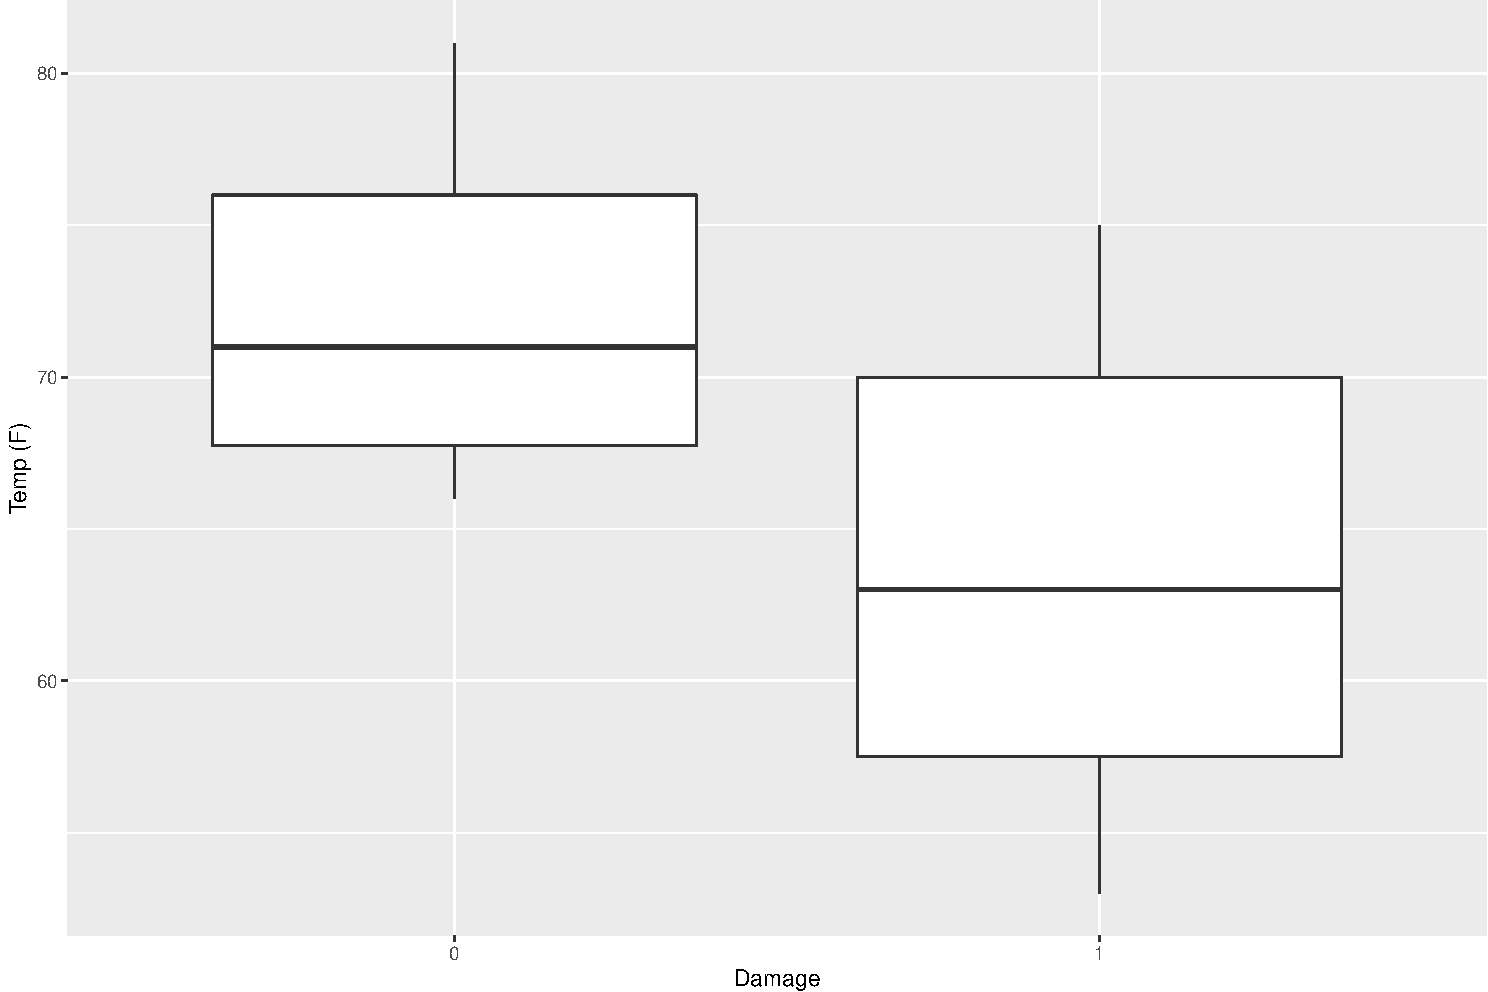
\includegraphics{9-logistic-regression_files/figure-beamer/unnamed-chunk-3-1.pdf}

\end{frame}

\begin{frame}{Linear models}
\protect\hypertarget{linear-models}{}

Why is \textbf{linear regression} not appropriate for this data?

\end{frame}

\begin{frame}{Beyond Linear Models}
\protect\hypertarget{beyond-linear-models}{}

While linear models are useful, they are limited when

\begin{enumerate}
\tightlist
\item
  the range of \(y_i\) is restricted (e.g., binary or count)
\item
  the variance of \(y_i\) depends on the mean
\end{enumerate}

\textbf{Generalized linear models} (GLMs) extend the linear model
framework to address both of these issues.

\end{frame}

\begin{frame}{Motivations and goals}
\protect\hypertarget{motivations-and-goals}{}

\begin{itemize}
\tightlist
\item
  We will revisit not just the challenger data, but other missions to
  understand the relationship between o-ring failure and temperature.
\item
  In order to understand this case study, we first need to learn about
  exponential families, generalized linear models, and logistic
  regression.
\end{itemize}

\end{frame}

\begin{frame}{Background}
\protect\hypertarget{background}{}

We need to introduce:

\begin{itemize}
\tightlist
\item
  exponential families
\item
  generalized linear models
\item
  and logistic regression
\end{itemize}

\end{frame}

\begin{frame}{Exponential Families}
\protect\hypertarget{exponential-families}{}

Any density that can be written in the form of equation
\ref{eqn:exponential} is called an \textbf{exponential family}.

\begin{align}
\label{eqn:exponential}
f(y; \theta, \phi) = \exp\left\{ \frac{y\theta - b(\theta)}{a(\phi)} + c(y,\phi) \right\},
\end{align}

where \(\theta\) and \(\phi\) are the \textbf{natural and dispersion
parameters}, respectively and \(a,b,c\) are functions.

\end{frame}

\begin{frame}{Connection to GLMs}
\protect\hypertarget{connection-to-glms}{}

In a GLM, pdfs or pmfs can be shown to be an exponential family using
equation\textasciitilde{}\ref{eqn:exponential}.

When doing this, it's important to identify the parameters of the
exponential family, namely:

\[\theta, \; \phi, \; a(\phi),\; b(\theta),\; c(y,\phi).\] Our overall
goal is to estimate \(\mu = E[Y \mid X].\)

\end{frame}

\begin{frame}{Connection to GLMs}
\protect\hypertarget{connection-to-glms-1}{}

\begin{align}
f(y; \theta, \phi) = \exp\left\{ \frac{y\theta - b(\theta)}{a(\phi)} + c(y,\phi) \right\},
\end{align}

\begin{itemize}
\item
  The natural parameter \(\theta\) is used to govern the shape of the
  density \(Y\mid X.\) Thus, \(\mu\) depends on \(\theta.\)
\item
  The dispersion parameter \(\phi\) is assumed known.
\item
  For GLM's, \(\eta = \beta^T X= \beta_1 X_1 + \ldots \beta_p X_p.\)
\end{itemize}

Our goal is to model a transformation of the mean \(\mu\) by a function
of \(X\):

\[g(\mu) = \eta(X).\]

\end{frame}

\begin{frame}{Generalized Linear Models}
\protect\hypertarget{generalized-linear-models}{}

Given covariates \(X\) and an outcome \(Y,\) a \textbf{generalized
linear model} is defined by three components:

\begin{enumerate}
\tightlist
\item
  a \textbf{random component}, which specifies a distribution for
  \(Y \mid X.\)
\item
  a \textbf{systematic component} that relates the parameter \(\eta\) to
  the covariates \(X\)
\item
  a \textbf{link function} that connects the random and systematic
  components
\end{enumerate}

\end{frame}

\begin{frame}{Exponential Families and GLMs}
\protect\hypertarget{exponential-families-and-glms}{}

We assume \(\mu = E[Y\mid X]\) and our goal is to estimate \(\mu.\)

\begin{itemize}
\tightlist
\item
  The \textbf{systematic component} relates \(\eta\) to \(X.\)
\end{itemize}

In a GLM, \[\eta = \beta^T X = \beta_1 X_1 + \ldots \beta_p X_p\]

The \textbf{link component} connects the \textbf{random} and
\textbf{systematic components}, via a link function \(g.\)

The link function provides a connection between \(\mu = E[Y\mid X]\) and
\(\eta.\)

\end{frame}

\begin{frame}{Exponential Families and GLMs}
\protect\hypertarget{exponential-families-and-glms-1}{}

\center
\Large

Let's look at an example to solidify our knowledge of exponential
families and GLM's.

\end{frame}

\begin{frame}{Bernoulli Example}
\protect\hypertarget{bernoulli-example}{}

Suppose \(Y \in \{ 0, 1\}\) and
\[Y\mid X \stackrel{iid}{\sim} \text{Bernoulli}(p).\]

Show that \(Y \mid X\) is in the exponential family, and provide the
respective parameters. Also, identify the link function g.

\end{frame}

\begin{frame}{Bernoulli Solution}
\protect\hypertarget{bernoulli-solution}{}

Note that:

\begin{align}
f(y) &= p^y(1-p)^{1-y} \\
&= \exp\{
y \log p + (1-y) \log(1-p)
\} \\
&= \exp\{
y \log ({\frac{p}{1-p}}) + \log(1-p) + 0
\} 
\end{align}

\end{frame}

\begin{frame}{Bernoulli Solution}
\protect\hypertarget{bernoulli-solution-1}{}

\begin{align}
f(y) &= \exp\{
y \log ({\frac{p}{1-p}}) + \log(1-p) + 0
\} 
\end{align}

\begin{itemize}
\item
  The natural parameter is \(\theta = \dfrac{p}{1-p}.\)
\item
  The mean is \(\mu = p,\) which implies that
  \(p = e^{\theta}/(1 + e^{\theta}).\)
\item
  This implies \(b(\theta) = -\log(1-p) = -\log(1 + e^{\theta}).\)
\item
  There is no dispersion parameter, so \(a(\phi) = 1\) and
  \(c(y,\phi) = 0.\)
\end{itemize}

\end{frame}

\begin{frame}{Bernoulli Solution}
\protect\hypertarget{bernoulli-solution-2}{}

\begin{align}
f(y) &= \exp\{
y \log ({\frac{p}{1-p}}) + \log(1-p) + 0
\} 
\end{align}

The link function is \[g(\mu) = \log(\frac{\mu}{1-\mu})\] such that we
model \[\log(\frac{\mu}{1-\mu}) = \text{logit}(\mu)= \beta^TX.\]

This is known as \textbf{logistic regression}, which is a GLM with the
\textbf{logit link}.

\end{frame}

\begin{frame}{Challenger Case Study}
\protect\hypertarget{challenger-case-study}{}

Let's return to the case study of the challenger, where

\begin{itemize}
\item
  The response is the damage to the o-ring (in each shuttle launch).
\item
  The covariate is the temperature (F) in each shuttle launch.
\end{itemize}

\end{frame}

\begin{frame}{Notation and Setup}
\protect\hypertarget{notation-and-setup}{}

\begin{itemize}
\item
  Let \(p_i\) be the probability that an o-ring \(i\) fails.
\item
  The corresponding \textbf{odds of failure} is \[\frac{p_i}{1-p_i}.\]
\end{itemize}

\end{frame}

\begin{frame}{Notation and Setup}
\protect\hypertarget{notation-and-setup-1}{}

\begin{itemize}
\item
  The probability of failure \(p_i\) is between \([0,1]\)
\item
  The odds of failure is any real number.
\end{itemize}

\end{frame}

\begin{frame}{Logistic Regression}
\protect\hypertarget{logistic-regression}{}

The response

\begin{align}
Y_i \mid p_i &\sim \text{Bernoulli}(p_i)
\end{align} for \(i=1,\ldots,n.\)

The logistic GLM writes that the logit of the probability \(p_i\) as
linear function of the predictor variable(s) \(x_i\):

\begin{align}
\text{logit}(p_i)  &:= \log(\frac{p_i}{1-p_i}) = \beta_0 + \beta_1x_i.
\end{align}

\end{frame}

\begin{frame}{Interpretation of Co-efficients}
\protect\hypertarget{interpretation-of-co-efficients}{}

\begin{itemize}
\item
  The regression coefficients \(\beta_0\), \(\beta_1\) are directly
  related to the log odds \(\log(\frac{p_i}{1-p_i})\) and not \(p_i.\)
\item
  For example, the intercept \(\beta_0\) is the
  \(\log(\frac{p_i}{1-p_i})\) for observation \(i\) when the predictor
  takes a value of 0.
\item
  The slope \(\beta_1\) refers to the change in the expected log odds of
  failure of an o-ring for a decrease in temperature.
\end{itemize}

\end{frame}

\begin{frame}{Intuition of Model}
\protect\hypertarget{intuition-of-model}{}

We assume our 23 data points are \textbf{conditionally independent}.

\[\text{Pr(failure = 1)} = \frac{\exp\{\beta_0 + \beta_1 \times \text{temp}\}}{1+ \exp\{\beta_0 + \beta_1 \times \text{temp}\}}\]
\begin{align}
&\text{failure}_1,\ldots, \text{failure}_{23} \mid \beta_0, \beta_1, \text{temp}_1,\ldots, \text{temp}_{23} \\
& \sim 
\prod_i 
\left(\frac{\exp\{\beta_0 + \beta_1 \times \text{temp}_i\}}{1+ \exp\{\beta_0 + \beta_1 \times \text{temp}_i\}}\right)^{\text{failure}_i} \\
&\times
\left(\frac{1}{1+ \exp\{\beta_0 + \beta_1 \times \text{temp}_i\}}\right)^{\text{1-failure}_i}
\end{align}

\end{frame}

\begin{frame}{Exercise}
\protect\hypertarget{exercise}{}

Assume that \(\log(\frac{p_i}{1-p_i}) = \beta_0 + \beta_1x_i.\)

Show that
\[p_i = \frac{e^{\beta_0 + \beta_1x_i}}{e^{\beta_0 + \beta_1x_i} + 1}.\]

This shows that logit function guarantees that the probability \(p_i\)
lives in \([0,1].\)

\end{frame}

\begin{frame}{Logistic Regression}
\protect\hypertarget{logistic-regression-1}{}

Recall that \begin{align}
Y_i \mid p_i &\sim \text{Bernoulli}(p_i)
\end{align} for \(i=1,\ldots,n.\)

\begin{align}
\text{logit}(p_i)  &:= \log(\frac{p_i}{1-p_i}) = \beta_0 + \beta_1x_i.
\end{align}

Note: This is the logistic GLM that we saw earlier. To perform logistic
regression in \texttt{R}, you can use the \texttt{glm} function with the
logit link.

\end{frame}

\begin{frame}{Bayesian Logistic Regression}
\protect\hypertarget{bayesian-logistic-regression}{}

\textbf{How can we build minimal Bayesian prior knowledge?}

\end{frame}

\begin{frame}{Priors on \(\beta_0\) and \(\beta_1\)}
\protect\hypertarget{priors-on-beta_0-and-beta_1}{}

Conjugate priors do not exists on \(\beta_0\) and \(\beta_1.\)

We will consider the following weakly informative priors:

\begin{align}
\beta_0 &\sim \text{Normal}(0,1000) \\
\beta_1 &\sim \text{Normal}(0,1000) \\
\end{align}

\end{frame}

\begin{frame}{Posterior sampling}
\protect\hypertarget{posterior-sampling}{}

Since we cannot find the posterior in closed form, we will resort to
MCMC to approximate inference regarding \(\beta_0, \beta_1.\)

We can do this easily using the \texttt{logitMCMC} function in the
\texttt{MCMCpack} R package.

This package implements a random walk Metroplis algorithm.

\end{frame}

\begin{frame}{The random walk metropolis algorithm}
\protect\hypertarget{the-random-walk-metropolis-algorithm}{}

\begin{itemize}
\item
  We saw the random walk metropolis algorithm in Module 6, slide 31.
\item
  For a different review of this method, there is a nice explanation of
  it here: \url{https://www.youtube.com/watch?v=U561HGMWjcw}
\item
  We don't need to code it up, as someone has written a nice package in
  R, but you could do this on your own if you wanted to.
\end{itemize}

\end{frame}

\begin{frame}[fragile]{Posterior sampling}
\protect\hypertarget{posterior-sampling-1}{}

\begin{Shaded}
\begin{Highlighting}[]
\KeywordTok{library}\NormalTok{(MCMCpack)}
\end{Highlighting}
\end{Shaded}

\begin{verbatim}
## Loading required package: coda
\end{verbatim}

\begin{verbatim}
## Loading required package: MASS
\end{verbatim}

\begin{verbatim}
## ##
## ## Markov Chain Monte Carlo Package (MCMCpack)
\end{verbatim}

\begin{verbatim}
## ## Copyright (C) 2003-2020 Andrew D. Martin, Kevin M. Quinn, and Jong Hee Park
\end{verbatim}

\begin{verbatim}
## ##
## ## Support provided by the U.S. National Science Foundation
\end{verbatim}

\begin{verbatim}
## ## (Grants SES-0350646 and SES-0350613)
## ##
\end{verbatim}

\begin{Shaded}
\begin{Highlighting}[]
\NormalTok{failure <-}\StringTok{ }\NormalTok{orings}\OperatorTok{$}\NormalTok{damage}
\NormalTok{temperature <-}\StringTok{ }\NormalTok{orings}\OperatorTok{$}\NormalTok{temp}
\NormalTok{output <-}\StringTok{ }\KeywordTok{MCMClogit}\NormalTok{(failure}\OperatorTok{~}\NormalTok{temperature, }
                    \DataTypeTok{mcmc=}\DecValTok{1000}\NormalTok{, }\DataTypeTok{b0=}\DecValTok{0}\NormalTok{, }\DataTypeTok{B0=}\FloatTok{0.001}\NormalTok{)}
\end{Highlighting}
\end{Shaded}

\end{frame}

\begin{frame}[fragile]{Traceplots}
\protect\hypertarget{traceplots}{}

\footnotesize

\begin{Shaded}
\begin{Highlighting}[]
\KeywordTok{plot}\NormalTok{(output)}
\end{Highlighting}
\end{Shaded}

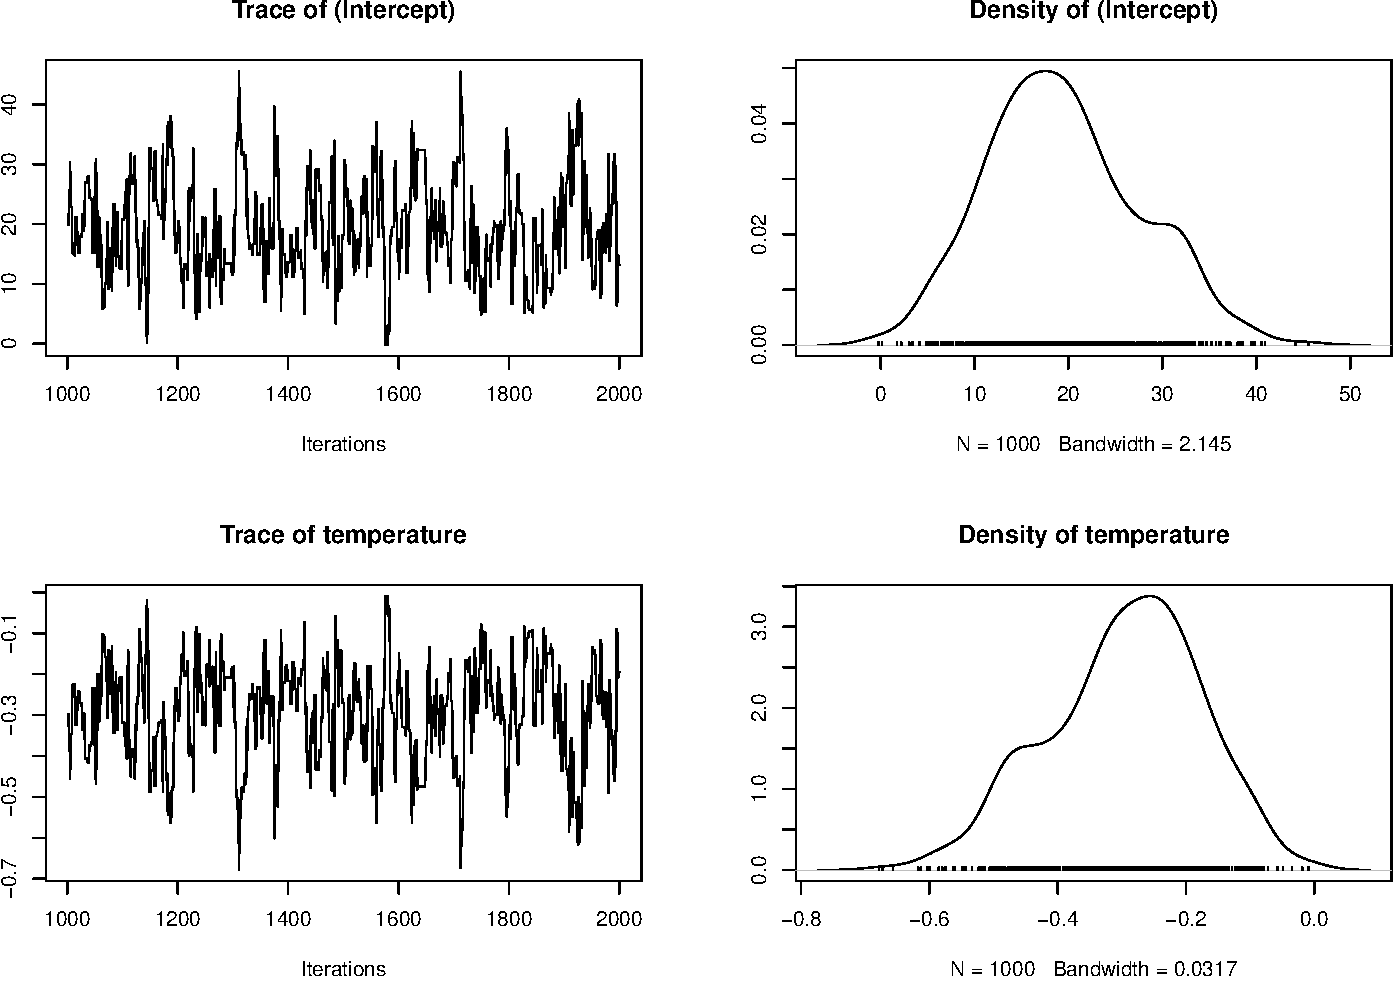
\includegraphics{9-logistic-regression_files/figure-beamer/unnamed-chunk-5-1.pdf}

\end{frame}

\begin{frame}[fragile]{Summary}
\protect\hypertarget{summary}{}

\footnotesize

\begin{Shaded}
\begin{Highlighting}[]
\KeywordTok{summary}\NormalTok{(output)}
\end{Highlighting}
\end{Shaded}

\begin{verbatim}
## 
## Iterations = 1001:2000
## Thinning interval = 1 
## Number of chains = 1 
## Sample size per chain = 1000 
## 
## 1. Empirical mean and standard deviation for each variable,
##    plus standard error of the mean:
## 
##                Mean     SD Naive SE Time-series SE
## (Intercept) 19.4239 8.1171 0.256684        0.88555
## temperature -0.2955 0.1191 0.003765        0.01309
## 
## 2. Quantiles for each variable:
## 
##                2.5%     25%     50%     75%    97.5%
## (Intercept)  5.3608 13.6196 18.7297 24.4156 36.08274
## temperature -0.5441 -0.3734 -0.2853 -0.2108 -0.09241
\end{verbatim}

\end{frame}

\begin{frame}{Simulating Posterior Prediction}
\protect\hypertarget{simulating-posterior-prediction}{}

Given a certain temperature, we can simulate the results of future space
shuttle launches using the posterior predictive distribution.

Suppose that on launch day, it's 80 degrees (F).

How would we simulate a predictive probability that a o-ring would fail?

\end{frame}

\begin{frame}[fragile]{Simulating Posterior Prediction}
\protect\hypertarget{simulating-posterior-prediction-1}{}

\begin{Shaded}
\begin{Highlighting}[]
\KeywordTok{library}\NormalTok{(boot)}
\end{Highlighting}
\end{Shaded}

\begin{verbatim}
## 
## Attaching package: 'boot'
\end{verbatim}

\begin{verbatim}
## The following objects are masked from 'package:faraway':
## 
##     logit, melanoma
\end{verbatim}

\begin{Shaded}
\begin{Highlighting}[]
\NormalTok{temp <-}\StringTok{ }\DecValTok{80}
\NormalTok{fail.prob <-}\StringTok{ }\KeywordTok{inv.logit}\NormalTok{(output[,}\DecValTok{1}\NormalTok{]}\OperatorTok{+}\StringTok{ }\NormalTok{temp}\OperatorTok{*}\NormalTok{output[,}\DecValTok{2}\NormalTok{])}
\NormalTok{y.pred <-}\StringTok{ }\KeywordTok{rbinom}\NormalTok{(}\DecValTok{2100}\NormalTok{, }\DataTypeTok{size=}\DecValTok{1}\NormalTok{, }\DataTypeTok{prob=}\NormalTok{fail.prob)}
\end{Highlighting}
\end{Shaded}

\end{frame}

\begin{frame}[fragile]{Simulating Posterior Prediction}
\protect\hypertarget{simulating-posterior-prediction-2}{}

\begin{Shaded}
\begin{Highlighting}[]
\KeywordTok{barplot}\NormalTok{(}\KeywordTok{table}\NormalTok{(y.pred))}
\end{Highlighting}
\end{Shaded}

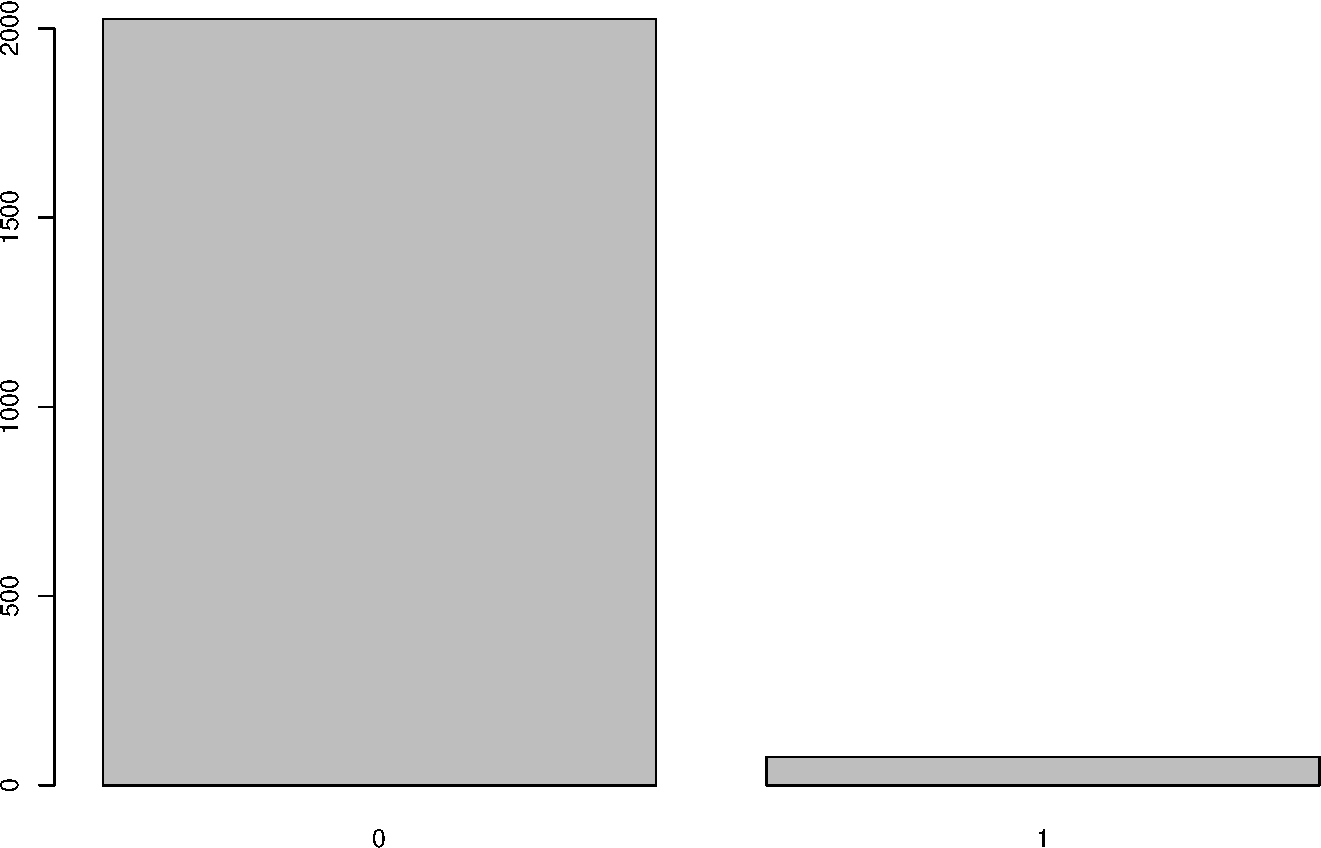
\includegraphics{9-logistic-regression_files/figure-beamer/unnamed-chunk-8-1.pdf}

\end{frame}

\begin{frame}{Your Turn}
\protect\hypertarget{your-turn}{}

Suppose that it's very cold, 20 F.

How would we simulate a predictive probability that a o-ring would fail?

\begin{itemize}
\tightlist
\item
  What does your group think intuitively?
\item
  Code up a simulation of a posterior prediction and what do you find?
\end{itemize}

\end{frame}

\begin{frame}{Summary}
\protect\hypertarget{summary-1}{}

\begin{itemize}
\tightlist
\item
  1986 Challenger explosion
\item
  Binary structure of the response data
\item
  Background: exponential families, generalized linear models (GLMs),
  logistic regression
\item
  Example on exponential families and GLMs
\item
  Bayesian logistic regression
\item
  Returning to the Challenger case study
\item
  What did you learn?
\end{itemize}

\end{frame}

\begin{frame}{Course evaluations}
\protect\hypertarget{course-evaluations}{}

\begin{itemize}
\tightlist
\item
  Course evaluations are available on github
\item
  There are instructions on how to fill out the course evaluations on
  Piazza
\item
  Please do also fill out the TA evaluations as well as they are
  eligible for awards that will help them in their careers
\item
  If there is 100 percent response, everyone in the class will receive 1
  point on their final grade. (We are currently just above 50 percent
  response.)
\item
  If there is something that has not been resolved in the course, please
  let me know so that it can be fixed. Kindly send myself (or your TA
  advocate an email regarding the issue).
\end{itemize}

\end{frame}

\begin{frame}{Gaussian Example}
\protect\hypertarget{gaussian-example}{}

Suppose \[Y\mid X \sim \text{Normal}(\mu, \sigma^2).\]

Then \[f(y) = \frac{1}{\sqrt{2\pi}\sigma}\exp \left\{
-\frac{1}{2\sigma^2} (y- \mu)^2
\right\}.\]

Show that \(Y \mid X\) is in the exponential family, and provide the
respective parameters.

\end{frame}

\begin{frame}{Gaussian Solution}
\protect\hypertarget{gaussian-solution}{}

\begin{align}
f(y)
&= (\sqrt{2\pi}\sigma)^{-1}\sigma\exp \left\{
-\frac{1}{2\sigma^2} (y- \mu)^2
\right\} \\
&= \exp\{\log(\sqrt{2\pi}\sigma)^{-1}\}
\exp \left\{
-\frac{1}{2\sigma^2} (y^2 - 2y\mu + \mu^2)
\right\} \\
&= \exp\{-\log(\sqrt{2\pi}) - \log\textcolor{blue}{\sigma} \}
\exp \left\{
 \frac{y\textcolor{blue}{\mu} -\textcolor{blue}{\mu^2/2}}{\sigma^2} - \frac{y^2}{2\textcolor{blue}{\sigma^2}}
\right\} \\
&=
\exp \{
\frac{y\textcolor{blue}{\mu} -\textcolor{blue}{\mu^2/2}}{\sigma^2}
- \frac{y^2}{2\textcolor{blue}{\sigma^2}}
-\log(\sqrt{2\pi}) - \log\textcolor{blue}{\sigma}
\}
\end{align}

The natural parameter \(\theta = \mu\) and \(b(\theta) = \theta^2/2.\)

The dispersion parameter is \(\phi = \sigma\) and
\(a(\phi) = \sigma^2.\)

Finally,
\(c(y,\phi) = \frac{y^2}{2\textcolor{blue}{\sigma^2}} - \log \phi - \log 2\pi.\)

The link function \(g(\mu) = \mu\) such that we model
\(\mu = \beta^TX.\)

\end{frame}

\end{document}
